\section{Introduction}
\label{sec:introduction}
The high-speed development of social networks brings explosive scale of information. The convenience of the social networks accelerates the diffusion of information. People create and publish messages without any limitations, which leads to the widespread dissemination of rumors in social networks \cite{DBLP:journals/corr/KurkaGZ15, DBLP:journals/csur/ZubiagaABLP18, DBLP:conf/sirocco/KostkaOW08, vosoughi2018spread}. Rumors usually appear with unjudged veracity and may include substantive misinformation, which may cause huge damage to the society. For instance, a large number of rumors arise during the CONVID-19 epidemic, such as ``More than ten thousand people die in Wuhan." and ``Liquor kills the virus.", causing great public panic. Therefore, defeating rumor is an urgent task for social networks. \textcolor{blue}{Considering the large volumes of data on social networks, manually defeating rumors is impossible. }

To automatically defeat rumors, many studies have been carried out. Generally speaking, the contributions are divided into two categories:  diffusion-based rumor source identification and content-based rumor detection. Diffusion-based rumor source identification aims to locate the source of the rumor by analyzing the infection status of the network with known topology \cite{DBLP:conf/sigmetrics/ShahZ10, DBLP:journals/tit/ShahZ11, DBLP:conf/kdd/LappasTGM10}. With rumor sources located, we effectively minimize the negative influence at the early stage of rumor diffusion. Content-based rumor detection aims to judge the veracity of microblog sequences that include the source microblog with its comments and retweets. As shown in Fig.\ref{fig:pipeline}, this task is a pipeline that is divided into 4 sub-tasks: rumor detection, rumor tracking, sentence classification, and veracity \cite{DBLP:journals/csur/ZubiagaABLP18, DBLP:conf/coling/KochkinaLZ18}. Rumor detection is the most popular task and it attracts enormous attention, which aims to classifier whether a microblogs sequence is a rumor. Many studies dedicated to this topic \cite{DBLP:conf/socinfo/ZubiagaLP17, DBLP:conf/www/Ma0W19,DBLP:conf/naacl/NguyenDCD19, DBLP:journals/corr/abs-1906-05659}. Sentence classification is to judge the emotion of a piece of microblog sentence \cite{DBLP:conf/semeval/EnayetE17, DBLP:conf/semeval/X17a, DBLP:conf/coling/ZubiagaKLPL16}. The possible emotions include: support, deny, query, and comments. The goal of the rumor veracity task is to judge if a piece of microblog tells the truth, which is a binary classification problem \cite{DBLP:conf/coling/KochkinaLZ18, DBLP:conf/acl/LiZS19, DBLP:conf/acl/KumarC19}. These three sub-tasks have attracted extensive attention in recent year. However, only a few studies have been proposed for rumor tracking task.

Rumor tracking is to collect related microblogs of a given rumor event. It is usually transformed into a binary classification problem that classifies the posts to be related or unrelated. Although there are several models for this task, some of the models are proposed a long time ago \cite{DBLP:conf/emnlp/QazvinianRRM11} and the others are not specifically for rumor tracking task \cite{DBLP:conf/www/ChengNB20}.
Consequently, considering the weakness of the existing work, we aim to design a specifically improved model for rumor tracking. 

The main contributions of this work are summarized a follows:
\begin{itemize}
	\item By exploring plenty of basic models, we proposed an aggregated model named ART to specifically solve the rumor tracking task. 
	\item We analyze the rumor tracking task and find suitable features and embedding methods. Also, we propose a voting based aggregation algorithm to aggregated basic models into a macrocosm.
	\item We conduct experiments on public benchmark datasets, and the experimental results show the rationality and superiority of ART.
\end{itemize}

The rest of this article is structured as follows. In Section \ref{sec:related}, we introduce important works related to ART. In Section \ref{sec:perliminary}, we introduce some notations and background knowledge of this work. Our proposed model ART is introduced in Section \ref{sec:model}. Then, Section \ref{sec:experiment} shows the experimental settings and results. Finally, we give the conclusion and future work in Section \ref{sec:conclusion}.

\begin{figure}[tbp]
	\hspace{0ex}
	\vspace{0ex}
	\centering
	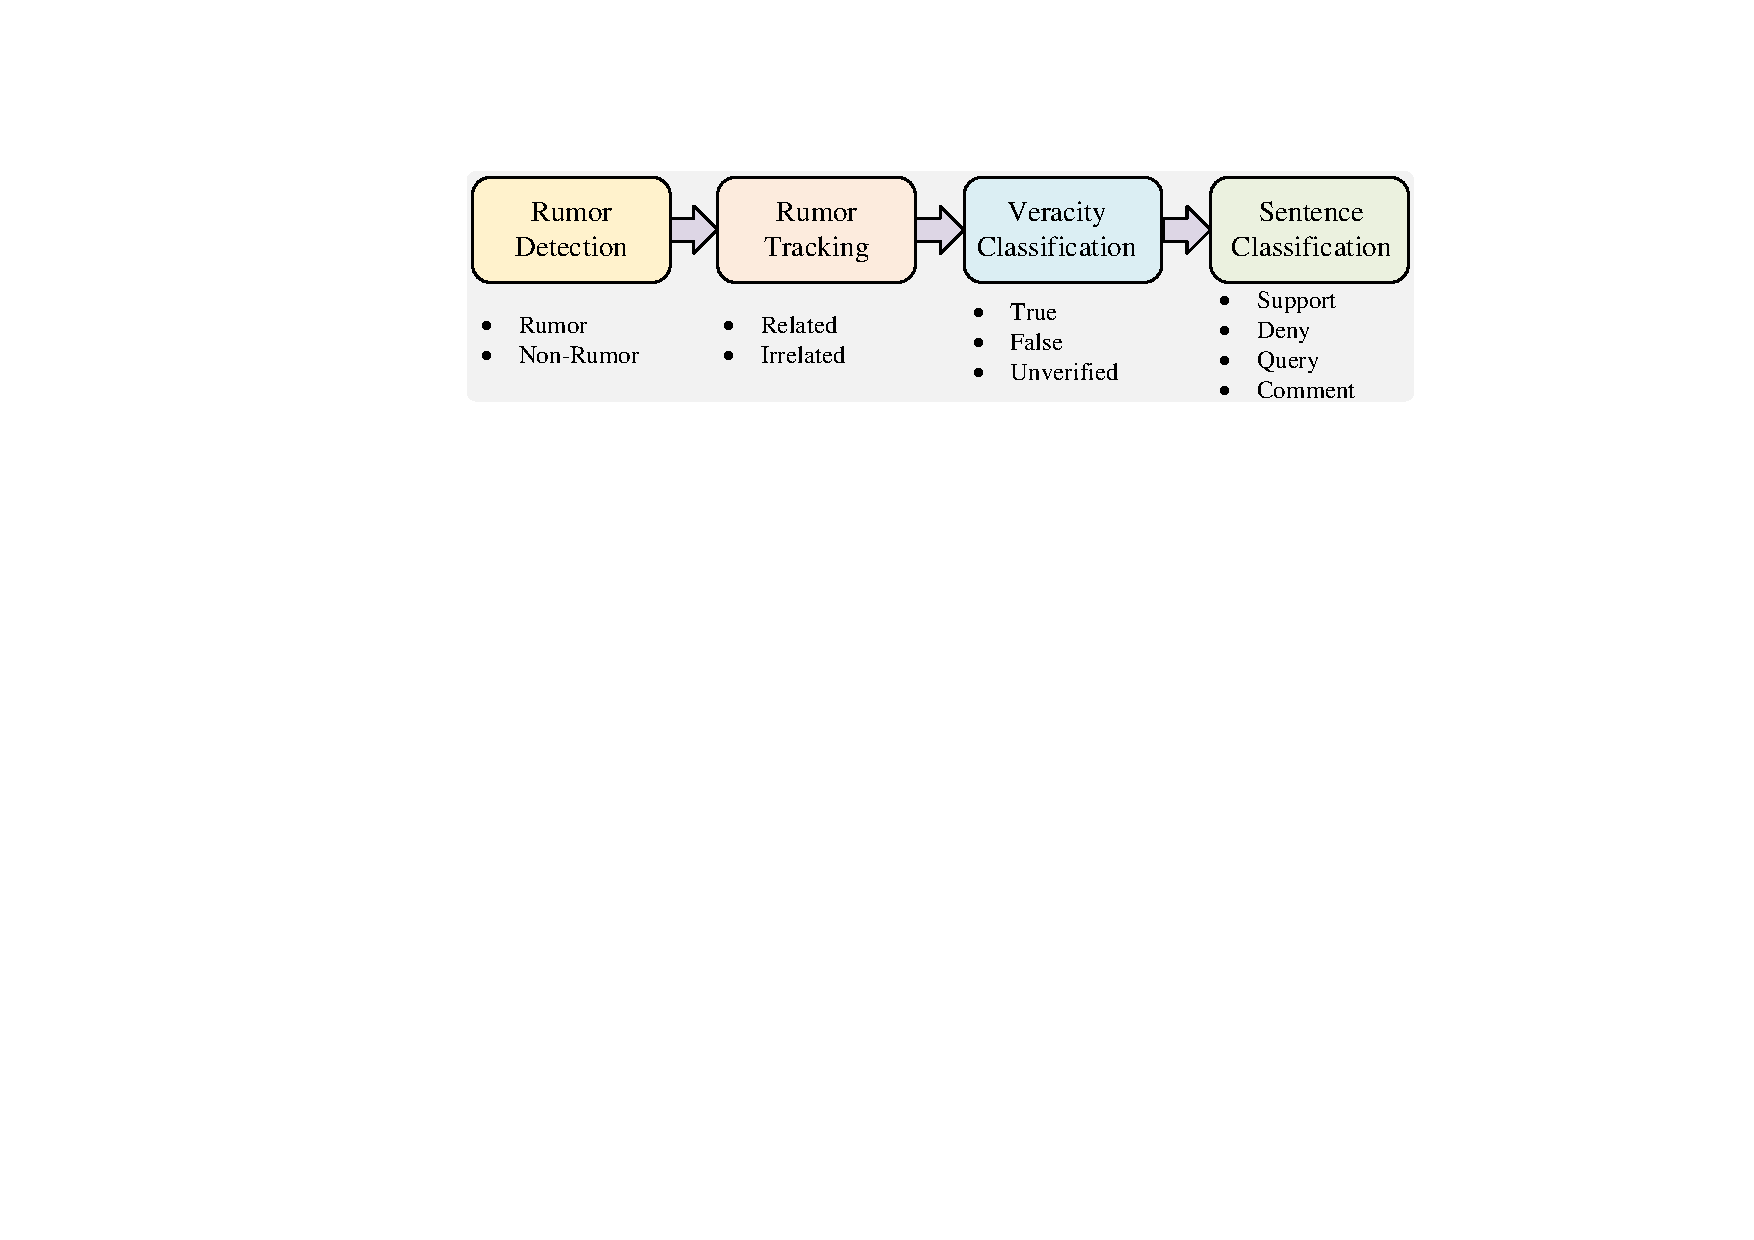
\includegraphics[width = \textwidth]{fig/pipeline}
	\caption{Pipeline of Rumor Detection Task}
	\label{fig:pipeline}
\end{figure}